The user here defines the structural model of the
building. The structural model is the part of the building designed
to resist the lateral loads. There are a number of backend
applications provided for this part of the workflow, each responsible
for defining the structural analysis model. The user can select the application to use from the drop-down menu at the top of this panel. As the user switches between applications,
the entry data changes to reflect the inputs each particular application requires. At present, there are two backend applications
available through the drop down menu: 

\begin{enumerate}
\item Multiple Degrees of Freedom (MDOF) (\Cref{sec:MDOF})
\item \texttt{OpenSees} (\Cref{sec:OpenSeesSIM})
\end{enumerate}

\subsection{Multiple Degrees of Freedom (MDOF)}\label{sec:MDOF}

This panel is provided for users to quickly create simple shear models
of a building. The panel, as shown in \Cref{fig:mdof} is divided
into 3 frames:
\begin{enumerate}
\item The top left frame allows the user to specify the number of stories and properties that are uniform for every story in the building. The following properties are available: floor weight, story height, and damping ratio for each story, and initial stiffness, yield strength, and hardening ratio for each direction in each story. Here, the 1 and 2 directions are orthogonal $x$ and $y$ axes in plan view.
\item The lower left frame allows the user to override the structural parameters above for individual stories.
\item The frame on the right is a graphical widget showing the current building. When entering data into the lower left frame, the stories corresponding to the data being modified are highlighted in red.
\end{enumerate}

\begin{figure}[!htbp]
  \centering {
    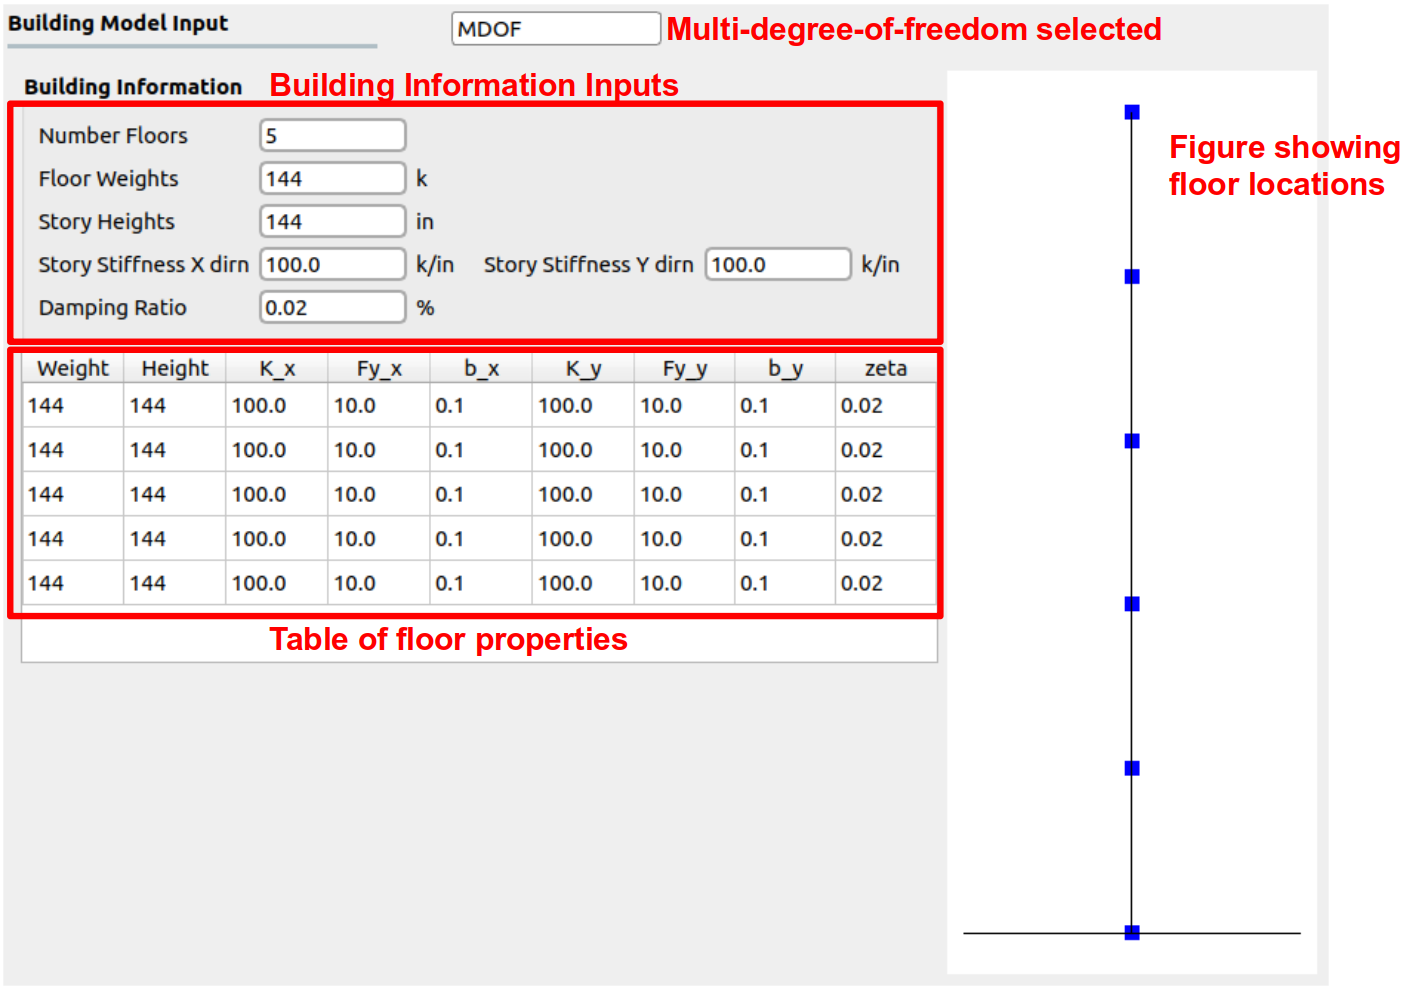
\includegraphics[width=0.8\textwidth]
    {usage/figures/mdof.png} }
  \caption{MDOF or Shear Building Model}
  \label{fig:mdof}
\end{figure}

Random Variables: Random Variables can be created by entering
a valid string instead of a number in the entry fields for any entry
except for the \emph{Number of floors}. The variable name entered will appear as
a Random Variable in the UQ panel and the user must specify its properties there.

\subsection{\texttt{OpenSees}}\label{sec:OpenSeesSIM}
This panel is for users who have an existing \texttt{OpenSees} model of a
building that performs a gravity analysis and now they wish to subject that
building model to one of the \texttt{EVT} options provided. The input panel
for this option is shown in \Cref{fig:figure3}. Users need to provide three pieces of information:
\begin{enumerate} 
\item Main OpenSees Script: The main script that contains the building
  model. This script should build a model and perform any gravity
  analysis of the building that is required before the event is
  applied.
\item Column Line of Nodes: A list of node numbers that define a column line of interest for which
  the responses will be determined. The column nodes should be in
  order from ground floor to roof. 
  
  The EDP workflow application\softwareSwitch{PBE}{}{, described
  in \Cref{sec:edp},} uses this information to determine nodes at which
  displacement, acceleration, and story drifts are calculated.
\item An entry for the dimension of the model (i.e., 2D or 3D). This
  information is used when ground motions are applied.
\end{enumerate}

\begin{figure}[!htbp]
  \centering {
    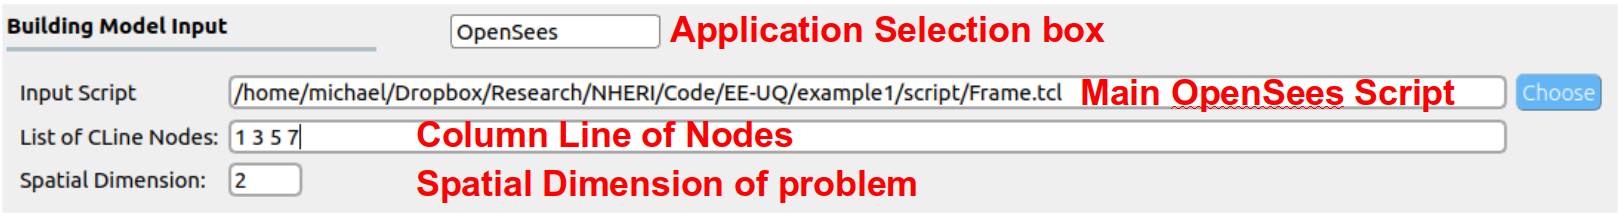
\includegraphics[width=0.8\textwidth]
    {usage/figures/openSees.png} }
  \caption{\texttt{OpenSees} Model}
  \label{fig:figure3}
\end{figure}

Random Variables: In \texttt{OpenSees} there is an option to set
variables to have certain values using the \texttt{pset} command, e.g
\texttt{pset a 5.0} will set the variable a to have a value 5 in an
\texttt{OpenSees} script. In \texttt{\getsoftwarename{}}, any variable
found in the main script to be set using the \texttt{pset} command
will be assumed to be a Random Variable. As such, when a new main
script is loaded all variables set with \texttt{pset} will appear as
Random Variables in the UQ panel.
